\chapter{One data-consistency step, and three seeds}\label{ch:consistency}

This is milestone M1b of the review, and it is the step that turned MAGIC-UNet from a tie with FISTA into a win. It is
our addition, not the paper's, so you should be able to derive it on a board.

\section{The problem it solves}

Chapter~\ref{ch:limits} ended with a strange fact: MAGIC-UNet is the best method where the measurement is silent (the
prior band) and the worst of the good methods where the measurement speaks (16.0\% in the measured band, against
FISTA's 9.1\%).

The reason is in how the two work. FISTA's loop compares its guess with the measurement at every iteration. MAGIC-UNet
looks at the measurement once and outputs a current. \textbf{Nothing forces that output to agree with what was measured.}
The check is simple: blur MAGIC-UNet's 0.5\um\ field back up to 3\um\ and compare with the real 3\um\ input. It misses by
17--33\%. The COMSOL truth itself, blurred the same way, misses by 10--17\%.

\section{Deriving the correction}

Call the network's field at 0.5\um\ $X$, the measurement $B$, and the blur between the two heights $H=e^{-k\,\Delta z}$.
We want a new field $X'$ that
\begin{itemize}
\item agrees with the measurement when blurred: $HX'\approx B$;
\item but stays close to the network's answer: $X'\approx X$.
\end{itemize}
Write both wishes as one cost, with a number $\mu$ that says how much the second matters:
\[
\min_{X'}\ |HX'-B|^2+\mu\,|X'-X|^2 .
\]
In Fourier space the blur is just a multiplication, so each frequency can be solved alone. Set the derivative to zero:
\[
H\,(HX'-B)+\mu\,(X'-X)=0
\quad\Longrightarrow\quad
X'=\frac{HB+\mu X}{H^2+\mu}.
\]
Rearranged into ``the old answer plus a correction'':
\[
\boxed{\;X'=X+\frac{H}{H^2+\mu}\,\bigl(B-HX\bigr)\;}
\]
The bracket is the mismatch: the measurement minus the network's field blurred up. The fraction turns that mismatch,
which lives at the measurement height, back into a change at 0.5\um.

\section{What it does at each frequency}

There is a second way to write the same formula that makes it easy to see:
\[
X'=w\cdot\frac{B}{H}+(1-w)\cdot X,\qquad w=\frac{H^2}{H^2+\mu}.
\]
$B/H$ is the plain inverse of the blur: what you get if you trust only the measurement. $X$ is what you get if you trust
only the network. $w$ is a dial between them, and it is different at every frequency:
\begin{itemize}
\item at low frequencies $H\approx1$, so $w\approx1$: \textbf{use the measurement};
\item at high frequencies $H\to0$, so $w\to0$: \textbf{keep the network}.
\end{itemize}
The changeover is where $H^2=\mu$.

\begin{figure}[H]
\centering
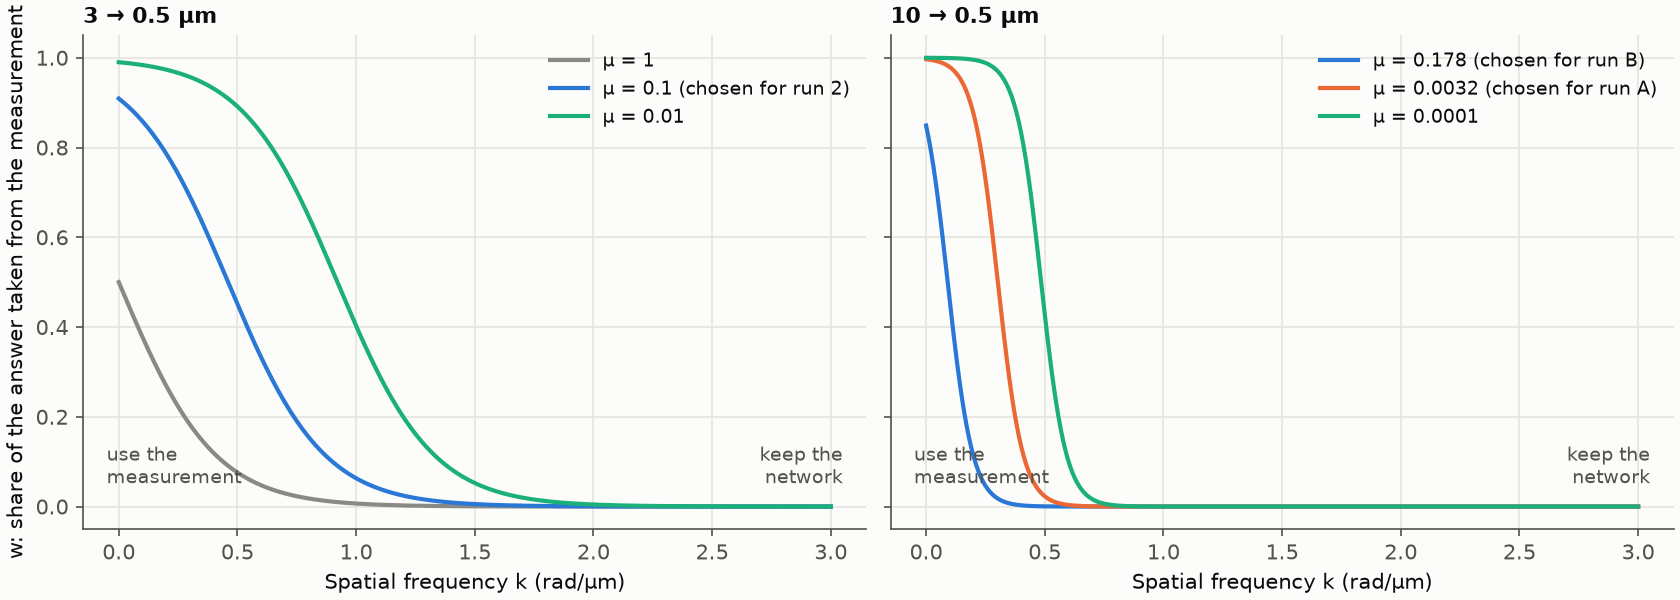
\includegraphics[width=0.95\textwidth]{late_dc_gain}
\caption{The dial $w$: how much of the final answer comes from the measurement, at each frequency. Left: 3\um\ to
0.5\um. Right: 10\um\ to 0.5\um, where the measurement only reaches the lowest frequencies.}
\label{fig:late_dc}
\end{figure}

\begin{keyidea}[Why this is the right kind of fix]
It gives each source of information the frequencies it is good at. The measurement decides the measured band. The
network's prior decides the band above it. That is exactly the split of Chapter~\ref{ch:limits}.
\end{keyidea}

\section{The code}

The whole step is six lines:

\begin{code*}{m12_common.py}
    n = np.asarray(x).shape[-1] + 2 * pad
    _, _, k = wavenumbers(n, dx)
    h = np.exp(-k * dz)
    fx, fb = padded_fft(x, pad), padded_fft(b, pad)
    return crop_ifft(fx + h / (h * h + mu) * (fb - h * fx), pad)
\end{code*}

The last line is the boxed formula. Before the transform the images are padded with 128 pixels of zeros on every
side, and cropped again afterwards. A Fourier transform treats an image as if it repeated forever, and without padding
the left edge would leak into the right.

Two tests check it against known answers: with exact data and $\mu\to0$ it returns the truth, and a prediction that
already agrees with the data is left unchanged.

\section{Choosing $\mu$, without touching COMSOL}

In the review's first diagnostic, three values of $\mu$ were tried directly on COMSOL. That is choosing on the test
data. Under the protocol, $\mu$ is chosen on \emph{simulated} images only, where the true target is known. For each of
17 values from $10^{-4}$ to 1, the corrected field is scored on 50 simulated layouts:

\begin{code*}{m1_rescore.py}
                corr = Corrector(pred.cpu().numpy(), b, z - 0.5, device)
                for m, mu in enumerate(mc.MU_GRID):
                    errors[i, m] = rel(corr(float(mu)), t)
\end{code*}

\begin{code*}{m1_rescore.py}
            mean = errors.mean((0, 2))
            best = int(np.argmin(mean))
            mu_curve[run].append(float(mc.MU_GRID[best]))
\end{code*}

This is repeated at every simulated standoff, which gives a curve $\mu(h)$. \code{Corrector} is the same formula on the
GPU, with the transforms done once so that 17 values are cheap:

\begin{code*}{m1_rescore.py}
    def __call__(self, mu):
        h = self.h
        out = torch.fft.irfft2(self.fx + h / (h * h + mu) * (self.fb - h * self.fx), s=(self.n, self.n))
        return out[..., mc.PAD:-mc.PAD, mc.PAD:-mc.PAD]
\end{code*}

\begin{center}
\small
\begin{tabular}{lcccccccc}
\toprule
Standoff (\textmu m) & 1 & 2 & 3 & 4 & 5 & 6 & 8 & 10 \\
\midrule
Best $\mu$ for run 2 & 0.32 & 0.18 & 0.1 & 0.056 & 0.01 & 0.0018 & 0.00056 & 0.00032 \\
\bottomrule
\end{tabular}
\end{center}

The best $\mu$ falls by about a thousand from 1 to 10\um. Two things drive it. A larger standoff makes $H$ smaller, so a
smaller $\mu$ is needed to keep the same dial setting. And outside its training range run 2 is poor, so the data
deserve more trust.

\section{Using the estimated height}

One thing is still missing. $H$ contains the standoff, and MAGIC-UNet is not supposed to be given the standoff. So the
correction uses the height of Chapter~\ref{ch:height}, read from the network's own current, and looks up $\mu$ on the
curve at that height:

\begin{code*}{m1_rescore.py}
                mu = mc.mu_at(row['h_star'], args.standoffs, mu_curve[run])
                fixed = Corrector(pred.cpu().numpy(), b, row['h_star'] - 0.5, device)(mu)
\end{code*}

\begin{code*}{m12_common.py}
def mu_at(h, standoffs, mus):
    """log10 mu linearly interpolated in h; held constant outside the simulated range (protocol M1b)."""
    return float(10 ** np.interp(h, np.asarray(standoffs, float), np.log10(np.asarray(mus, float))))
\end{code*}

So the full pipeline is: network $\to$ current $\to$ field at 0.5\um\ $\to$ read $h^\ast$ $\to$ one correction at $h^\ast$.
Nothing in it uses the true standoff.

\section{The result}

\begin{center}
\small
\begin{tabular}{lcccc}
\toprule
COMSOL, 3\um\ to 0.5\um, 15 pairs & Raw & Measured band & Prior band & Low-passed \\
\midrule
MAGIC-UNet run 2 & 27.0\% & 16.0\% & 14.6\% & 22.0\% \\
\quad + correction at the true height & 24.3\% & 10.9\% & 14.6\% & 18.5\% \\
\quad + correction at $h^\ast$ (standoff not given) & \textbf{24.3\%} & 11.0\% & 14.6\% & 18.5\% \\
FISTA, 1{,}000 iterations & 26.7\% & 9.1\% & 19.3\% & 21.9\% \\
FISTA, 925 iterations (the baseline from Ch.~\ref{ch:fista_depth}) & 26.9\% & & & \\
\bottomrule
\end{tabular}
\end{center}

\begin{keyidea}[It did exactly what the derivation promised]
The measured-band error fell from 16.0\% to 11.0\%. The prior-band error did not move: 14.6\% before and after. Not
knowing the height cost nothing here (24.3\% both ways), because the read-out at 3\um\ is good.
\end{keyidea}

On simulation the correction lowers the error at every standoff for both runs (at 3\um: 15.1\% to 13.7\% for run 2), and
on COMSOL it helps on all 40 rows that were scored.

\begin{careful}[An honest correction]
The review's first diagnostic gave 24.2\% on the two local configurations, with $\mu$ picked from three values on that
test data. Like for like, with $\mu$ from simulation, the same two configurations give 25.1\%. So choosing on the test
data had made the number 0.9 points too good. Small, but it is exactly the effect the protocol exists to prevent.
\end{careful}

\section{Three seeds}

A trained network depends on random numbers: the starting weights, the order of the batches, the noise drawn in
training. The \emph{seed} fixes them. Change the seed and you get a slightly different network. So far every network had
one seed, and a difference between two methods could simply be luck.

Two more copies of run 2 were trained, identical except for the seed. And \emph{before} they finished, the rule for
reading them was written down (amendment A4):

\begin{keyidea}[The rule]
``MAGIC-UNet beats FISTA on a set of pairs'' may be written only if \textbf{all three seeds} score below FISTA on that
set. If even one does not, the result is written as ``not distinguishable on this test set'', whatever the average
says. FISTA has no seed: it gives the same answer every time.
\end{keyidea}

\begin{center}
\small
\setlength{\tabcolsep}{4pt}
\begin{tabular}{llcccccl}
\toprule
 & Set & Seed 0 & Seed 1 & Seed 2 & FISTA-1000 & FISTA-925 & Verdict \\
\midrule
Raw & 15 pairs & 27.0\% & 27.2\% & 26.7\% & 26.7\% & 26.9\% & not distinguishable \\
Raw & \code{IC_4um} & 29.6\% & 29.8\% & 32.6\% & 27.2\% & 27.2\% & not distinguishable \\
\midrule
Corrected & 15 pairs & 24.3\% & 24.5\% & 24.5\% & 26.7\% & 26.9\% & \textbf{beats FISTA} \\
Corrected & C1 family & 23.8\% & 23.7\% & 22.9\% & 26.6\% & 26.8\% & \textbf{beats FISTA} \\
Corrected & \code{IC_4um} & 26.4\% & 27.5\% & 30.9\% & 27.2\% & 27.2\% & not distinguishable \\
\bottomrule
\end{tabular}
\end{center}

The rule was first applied against FISTA-1000. Against FISTA-925, the baseline of Chapter~\ref{ch:fista_depth}, every
verdict is the same. Read the last row carefully. Seed 0, the original run 2, is 0.8 points better than FISTA on \code{IC_4um}. Seed 2 is 3.6
points worse. The earlier ``win'' on that coil was luck. \code{IC_4um} is one shape with three component images, and its
seeds spread over 4.4 points, more than any margin on it.

\begin{keyidea}[The fair summary at 3\um, and the one to use in your report]
With one data-consistency step, MAGIC-UNet beats a converged FISTA on the 15 pairs and on the C1-family coils, for
every seed, without being told the standoff: 24.3--24.5\% against 26.9\% for FISTA at its best depth (26.7\% at
1{,}000 iterations). On \code{IC_4um} the two are \textbf{not
distinguishable}. The paper's network on its own ties FISTA.
\end{keyidea}

\begin{defend}[If your professor asks: is the data-consistency step from the paper?]
No. It is our addition and must be labelled so every time. It is one linear step with one number $\mu$, chosen on
simulated data, at a height the network estimates itself. It changes only the frequencies the measurement carries.
\end{defend}

\begin{defend}[If your professor asks: why not put FISTA's data consistency inside the network?]
That is the method the review recommends for the future: a learned current prior inside several data-consistency
steps, with a search over height. One step applied afterwards was the cheapest possible test of whether that direction
is right. It was.
\end{defend}

\begin{defend}[If your professor asks: why only three seeds?]
Each run takes 4 to 8 hours on the one GPU. Three is the minimum that lets a rule like ``all seeds below the
baseline'' mean something, and the rule was written before the seeds finished.
\end{defend}
